% 3-minute presentation, 4 slides, following the professor's
% recommended structure:
%   Slide 1: problem + dataset + goal + sample images
%   Slide 2: PCA / LDA / t-SNE side-by-side -- structure of the data
%   Slide 3: models compared and our proposed modification
%   Slide 4: results + conclusion + one limitation + one future direction
\documentclass[10pt,aspectratio=169]{beamer}
\usetheme{default}
\usecolortheme{default}
\setbeamertemplate{navigation symbols}{}
\setbeamertemplate{footline}{}
\setbeamertemplate{headline}{}

% --- beige / white palette ---
\definecolor{SlideBeige}{RGB}{245,240,230}
\definecolor{SlideBrown}{RGB}{90,70,50}
\definecolor{SlideAccent}{RGB}{140,100,60}

\setbeamercolor{background canvas}{bg=SlideBeige}
\setbeamercolor{frametitle}{fg=black,bg=SlideBeige}
\setbeamercolor{title}{fg=black}
\setbeamercolor{subtitle}{fg=black}
\setbeamercolor{author}{fg=black}
\setbeamercolor{institute}{fg=black}
\setbeamercolor{normal text}{fg=black}
\setbeamercolor{itemize item}{fg=black}
\setbeamercolor{itemize subitem}{fg=black}
\setbeamercolor{structure}{fg=black}

\setbeamerfont{frametitle}{size=\Large,series=\bfseries}
\setbeamerfont{title}{size=\LARGE,series=\bfseries}

% thin rule under frame title
\addtobeamertemplate{frametitle}{}{%
  \vspace{-4pt}\textcolor{black}{\hrule height 0.4pt}\vspace{4pt}}
\usepackage{booktabs}
\usepackage{graphicx}
\graphicspath{{figures/}}

\title{CNN Architectures for Image Classification}
\subtitle{MNIST, CIFAR-10 \& a channel-attention residual variant}
\date{}
\author{Srinidhi Narla \& Pranav Cheedalla}
\institute{Department of Computer Science, UT Dallas \\ CS 4375.002, Spring 2026}

\begin{document}

\begin{frame}
\titlepage
\end{frame}

% =====================================================================
% Slide 1 -- problem, dataset, goal, with sample images
% =====================================================================
\begin{frame}{Problem, datasets, and goal}
\begin{columns}[T,onlytextwidth]
\begin{column}{0.52\linewidth}
\textbf{Task.} 10-class image classification.\\[2pt]
\textbf{Datasets.}
\begin{itemize}
  \item \textbf{MNIST} -- handwritten digits, $28{\times}28$ grayscale,
    60k train / 10k test, 10 classes (0--9).
  \item \textbf{CIFAR-10} -- natural objects, $32{\times}32$ RGB,
    50k train / 10k test, 10 classes (airplane, car, bird, cat, deer,
    dog, frog, horse, ship, truck).
\end{itemize}
\textbf{Goal.} Compare seven CNN architectures (one is our own
modification of ResNet-18) under a single training pipeline using
accuracy, macro precision/recall/F1, and AUROC.
\end{column}
\begin{column}{0.45\linewidth}
\centering
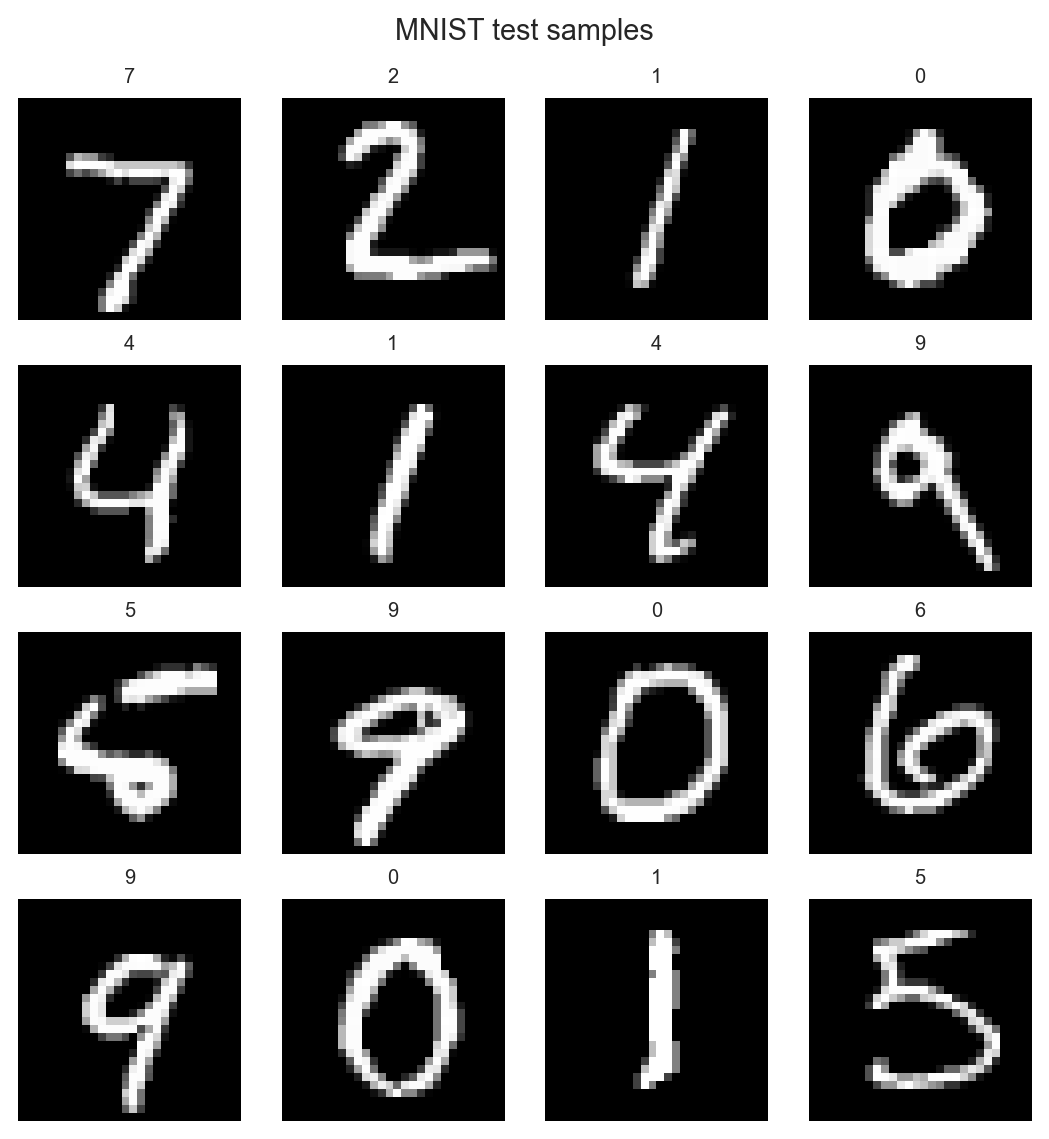
\includegraphics[width=\linewidth]{samples_mnist.png}\\[2pt]
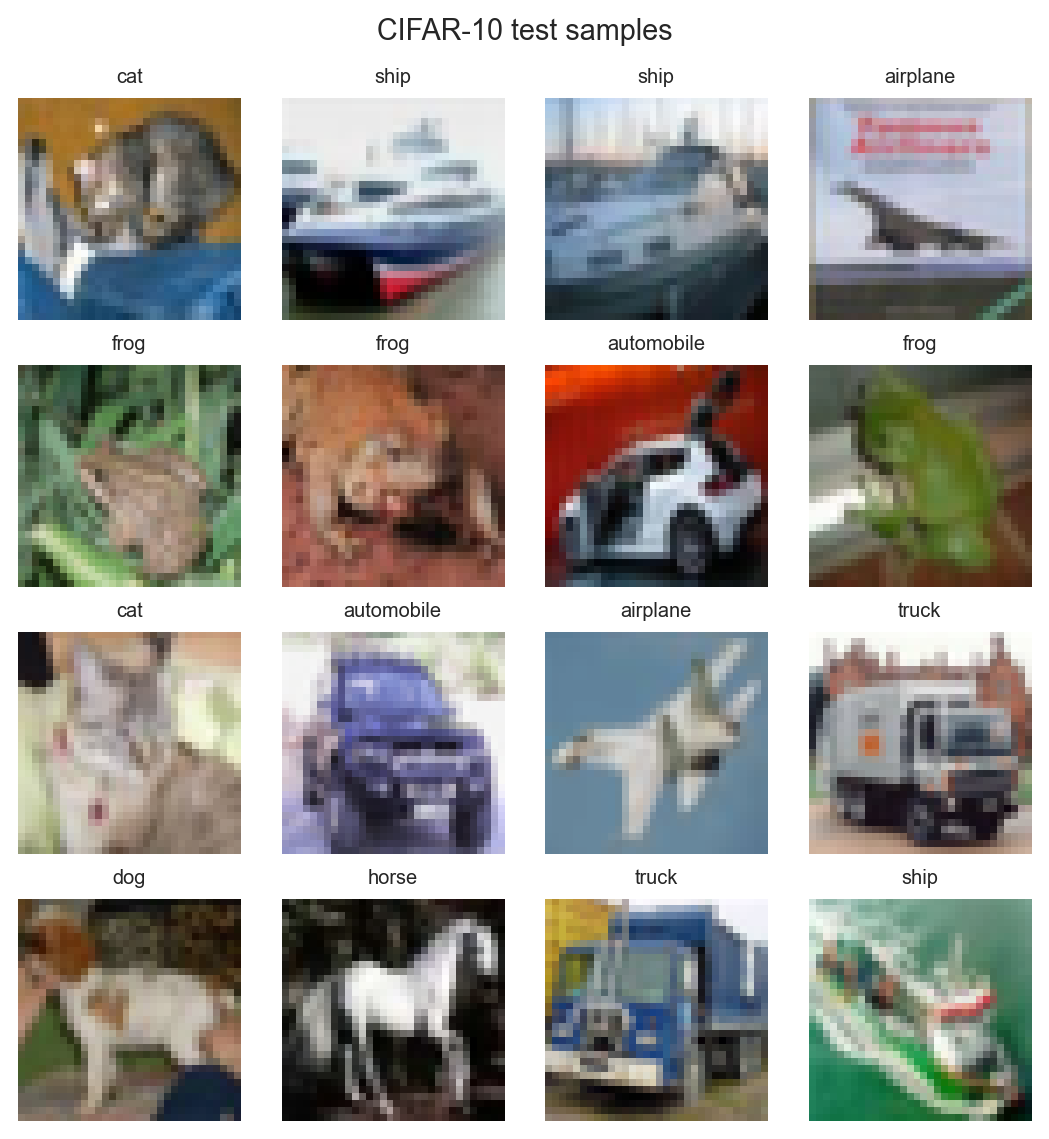
\includegraphics[width=\linewidth]{samples_cifar10.png}
\end{column}
\end{columns}
\end{frame}

% =====================================================================
% Slide 2 -- PCA / LDA / t-SNE on the data
% =====================================================================
\begin{frame}{Class structure: PCA \(\to\) LDA \(\to\) t-SNE}
\begin{columns}[T,onlytextwidth]
\begin{column}{0.5\linewidth}
\centering
\textbf{MNIST raw pixels}\\
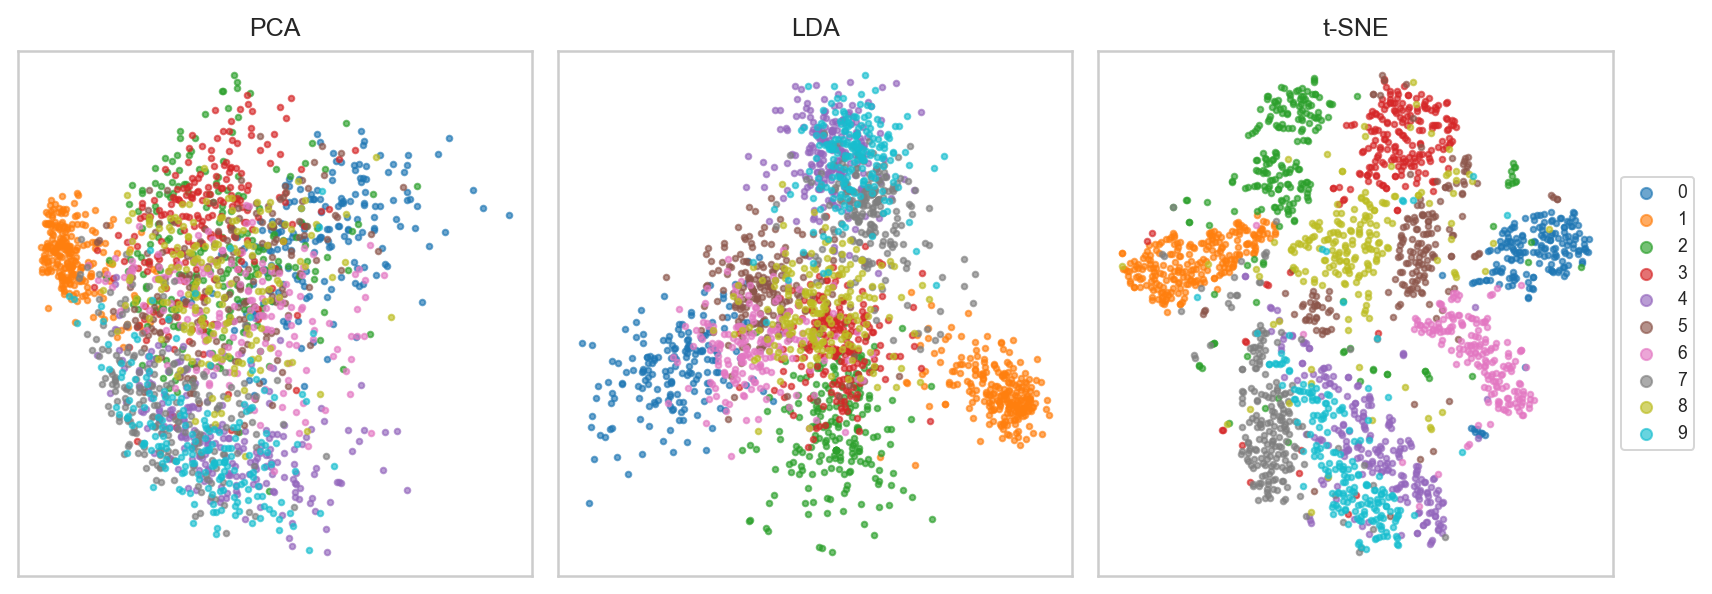
\includegraphics[width=\linewidth]{viz_raw_mnist.png}
\end{column}
\begin{column}{0.5\linewidth}
\centering
\textbf{CIFAR-10 raw pixels}\\
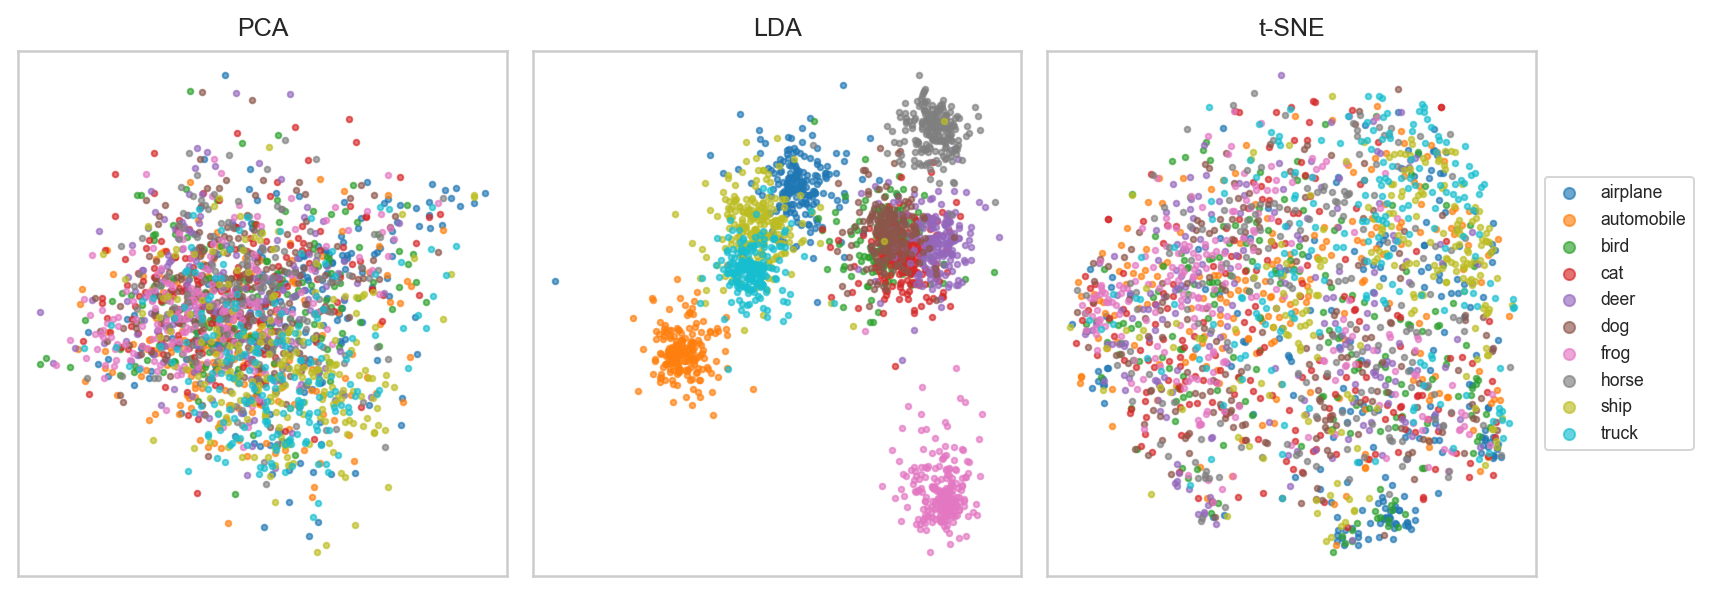
\includegraphics[width=\linewidth]{viz_raw_cifar10.png}
\end{column}
\end{columns}
\vspace{4pt}\small
\textbf{Takeaway.} MNIST classes form clear clusters even in raw
pixel space (LDA separates all 10 digits in 2D) --- this explains
why even a flat MLP scores 99\%. CIFAR-10 is the opposite: all
projections collapse into one overlapping cloud. Every percentage
point above 50\% on CIFAR-10 requires spatial feature learning that
only convolution can provide.
\end{frame}

% =====================================================================
% Slide 3 -- models compared and the proposed modification
% =====================================================================
\begin{frame}{Models compared, and our modification}
\begin{columns}[T,onlytextwidth]
\begin{column}{0.46\linewidth}
\textbf{Seven architectures, identical training recipe.}
\vspace{4pt}\\
\begin{tabular}{ll}
\toprule
\textbf{Model} & \textbf{Family} \\
\midrule
MLP             & baseline, no spatial bias \\
SimpleCNN       & 2 conv + 2 FC \\
LeNet-5         & classic 1998 CNN \\
AlexNet$^*$     & 5 conv + 3 FC \\
VGG-11$^*$      & deep $3{\times}3$ + BatchNorm \\
ResNet-18$^*$   & residual, 4 stages \\
\textbf{SE-ResNet-Lite} & \textbf{ours} \\
\bottomrule
\end{tabular}\\[3pt]
\small $^*$ Adapted for $32{\times}32$ inputs.
\end{column}
\begin{column}{0.5\linewidth}
\textbf{Our novel architecture --- SE-ResNet-Lite.}
\begin{itemize}\small
  \item Take ResNet-18 as the backbone.
  \item Insert a \textbf{Squeeze-and-Excitation block} inside every
    residual block. SE = global-pool \(\to\) 2-layer MLP \(\to\)
    sigmoid \(\to\) per-channel gating.
  \item Replace the stem with a \textbf{depthwise-separable}
    $3{\times}3$ DW \(\to\) $1{\times}1$ PW.
  \item Net parameter overhead vs ResNet-18: \textbf{$<\!1\%$}.
\end{itemize}
\vspace{3pt}\small
\textbf{Hypothesis.} Channel attention boosts accuracy; the lighter
stem keeps the parameter budget essentially fixed.
\end{column}
\end{columns}
\end{frame}

% =====================================================================
% Slide 4 -- results, conclusion, limitation, future work
% =====================================================================
\begin{frame}{Results and conclusions}
\begin{columns}[T,onlytextwidth]
\begin{column}{0.56\linewidth}
\small
\begin{tabular}{lrrr}
\toprule
\textbf{Model} & \textbf{MNIST acc} & \textbf{CIFAR-10 acc} & \textbf{F1} \\
\midrule
MLP             & 99.03\% & 50.18\% & 0.493 \\
SimpleCNN       & 99.46\% & 75.34\% & 0.752 \\
LeNet-5         & 99.31\% & 61.02\% & 0.606 \\
AlexNet         & 99.57\% & 84.03\% & 0.840 \\
VGG-11          & 99.62\% & 89.48\% & 0.895 \\
ResNet-18       & 99.65\% & 91.38\% & 0.914 \\
\textbf{SE-ResNet-Lite} & \textbf{99.70\%} & \textbf{92.67\%} & \textbf{0.927} \\
\bottomrule
\end{tabular}
\vspace{6pt}\\
\textbf{Key findings.}
\begin{itemize}\small
  \item Architecture barely matters on MNIST (0.67 pp spread); it
    matters enormously on CIFAR-10 (42.5 pp spread, MLP to SE-ResNet-Lite).
  \item Residual connections outperform VGG-11 by 1.9 pp at similar
    parameter count --- skip connections are doing real work, not just
    adding depth.
  \item SE-ResNet-Lite tops all models on \emph{both} datasets at
    $<\!1\%$ parameter overhead. The gain is most visible on
    \emph{cat}/\emph{dog}, where texture cues matter most.
\end{itemize}
\end{column}
\begin{column}{0.42\linewidth}
\centering
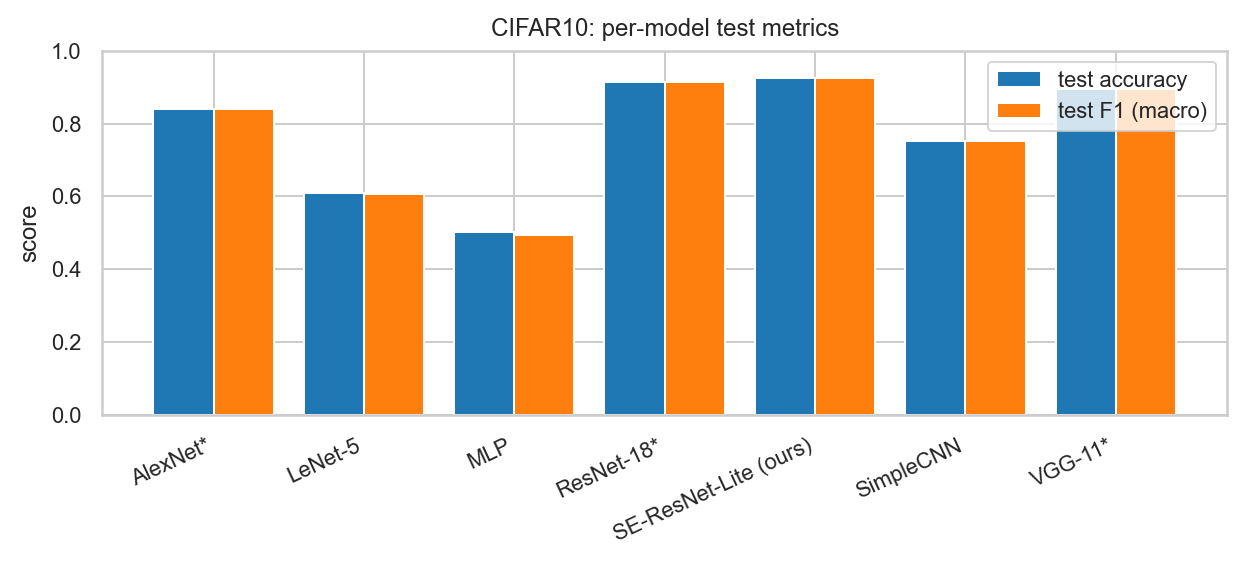
\includegraphics[width=\linewidth]{compare_cifar10.png}\\[3pt]
\small\textbf{Limitation.} Single random seed --- 1--2 pp differences
need multiple runs to be statistically meaningful.\\[3pt]
\textbf{Future work.} Ablate SE-only vs DW-stem-only; sweep
reduction ratio $r$; test on Tiny ImageNet.
\end{column}
\end{columns}
\end{frame}

\end{document}
